\begin{figure}[t]
\centering
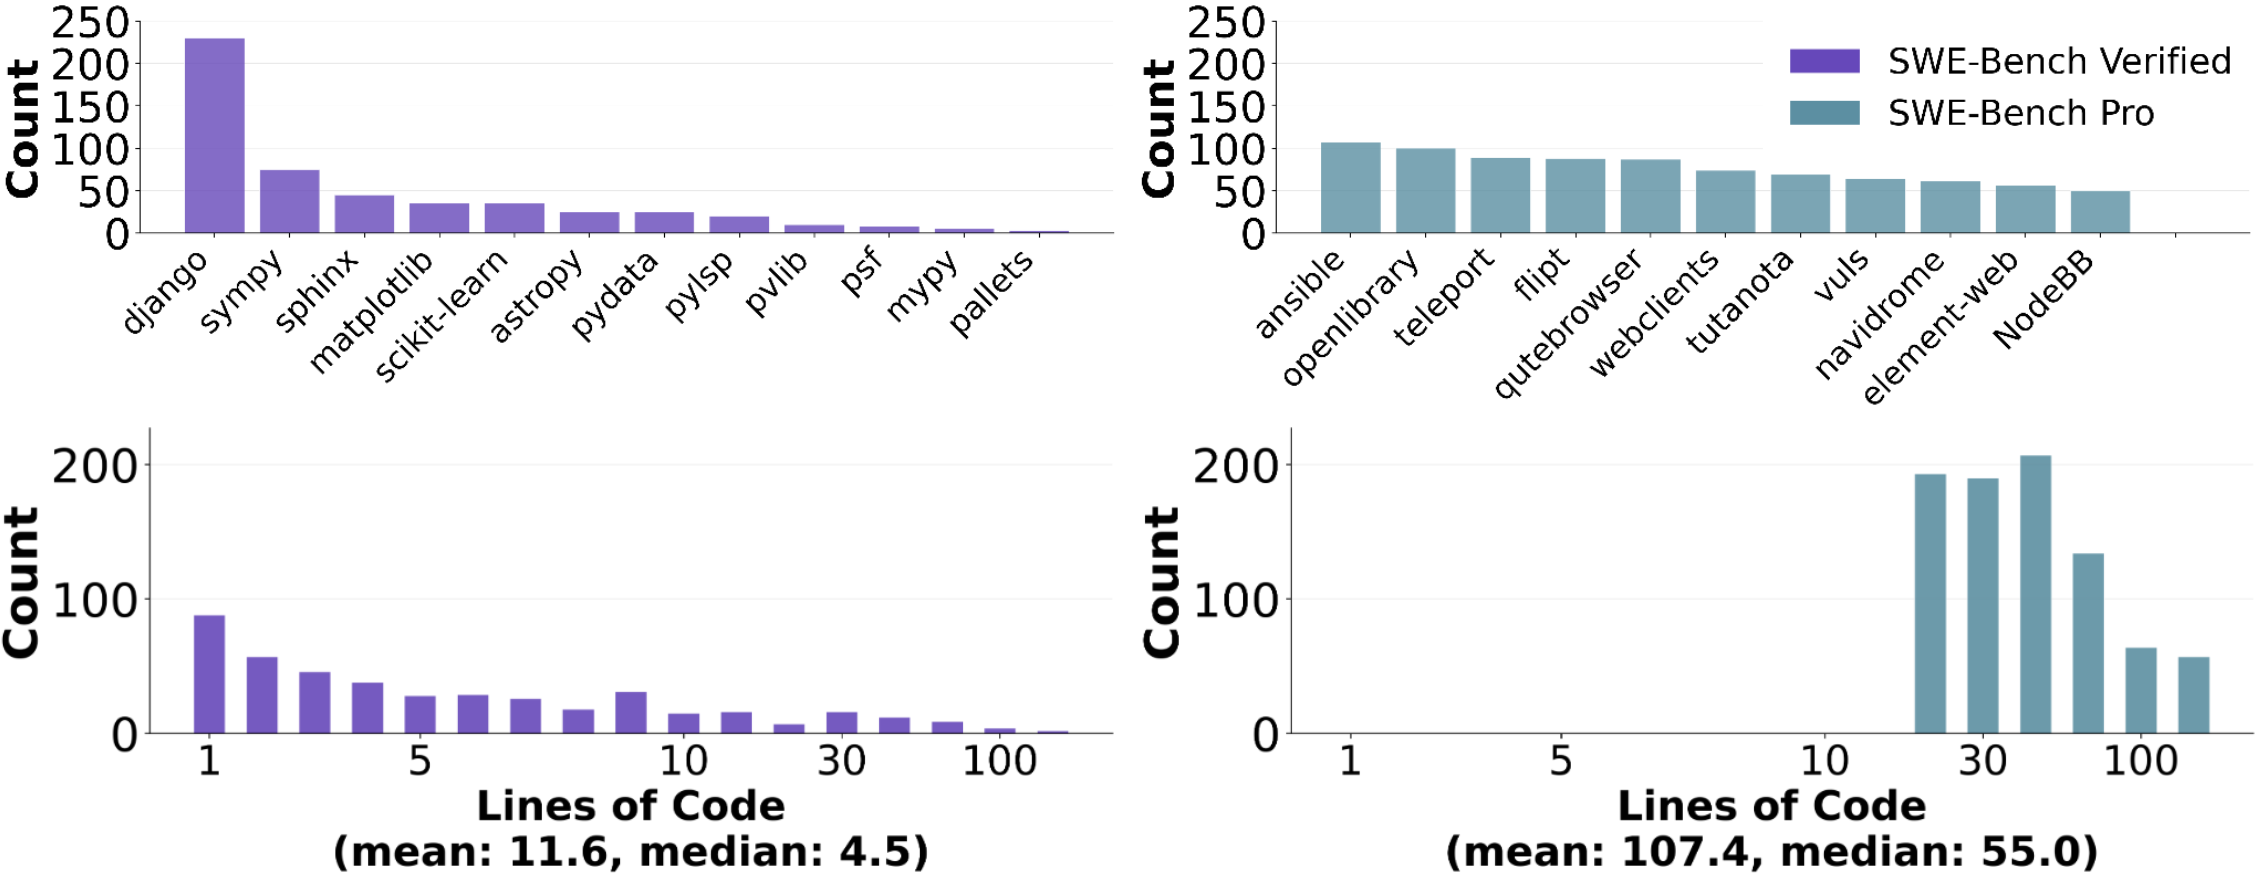
\includegraphics[width=\textwidth]{images/Figure_1_large.png}
\caption{Patches on \benchmarkname~are larger, more challenging, and require expert knowledge about a variety of topics. Patches are generated with SWE-Agent \cite{yang2024sweagent} and evaluated on the public subset of \benchmarkname.}
\label{fig:languages_repos}
\end{figure}

\section{Dataset Creation}

\begin{figure}[t]
\centering
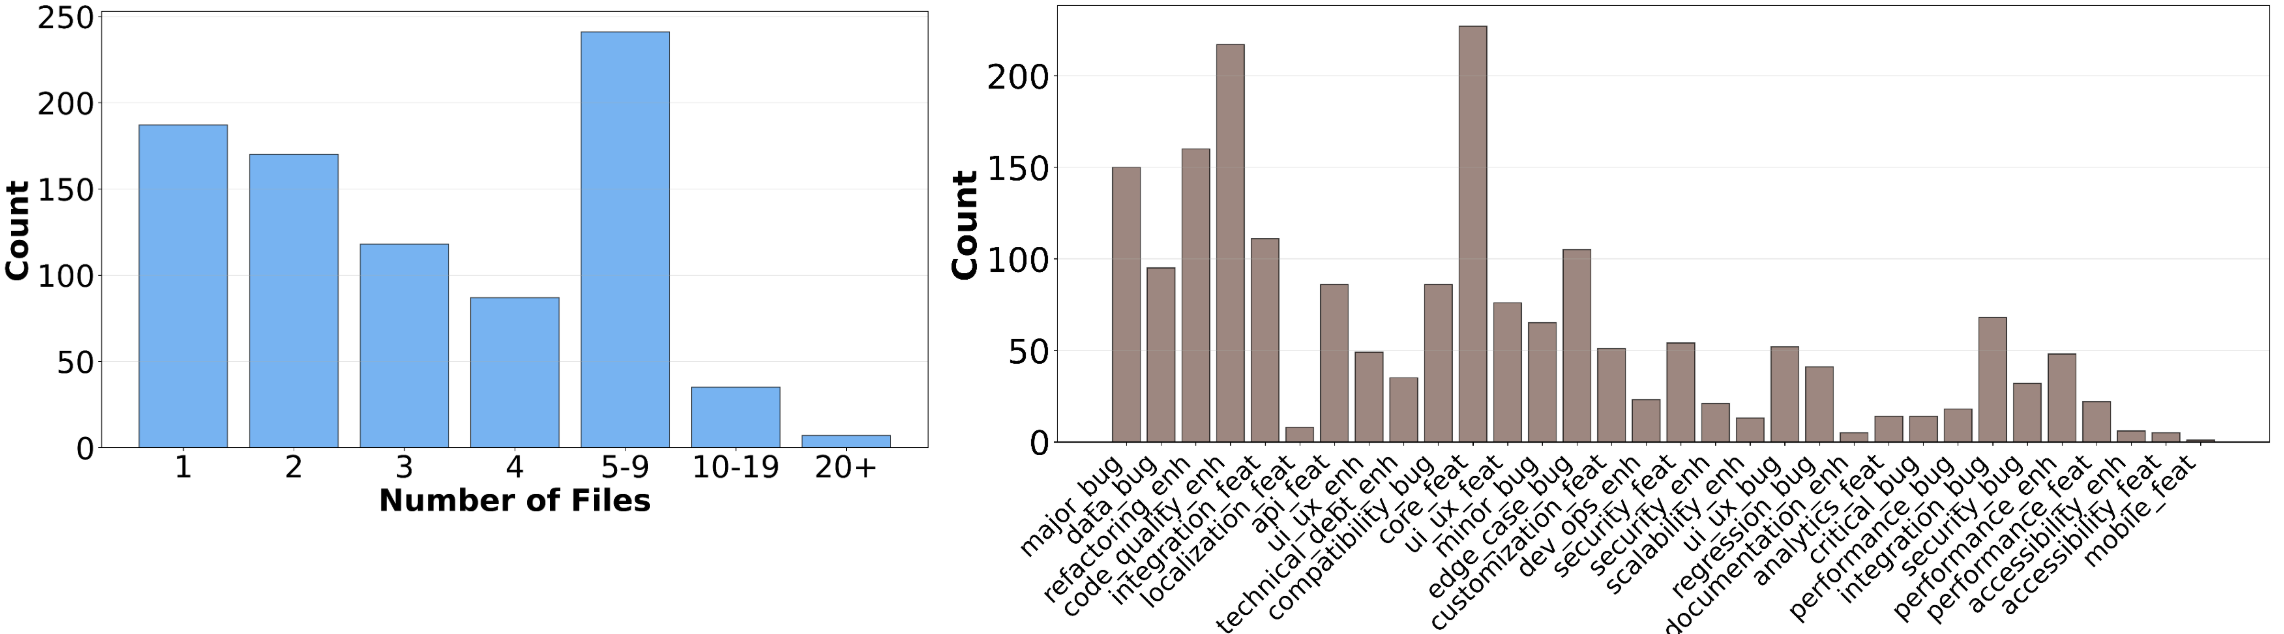
\includegraphics[width=\textwidth]{images/fies_and_categories.png}
\caption{Distributions in the public set of \benchmarkname. \benchmarkname~contains complex, long-horizon tasks involving several files and across a variety of task types. We include a diverse selection of feature requests as well as bug fixes, across optimization, security, UI/UX, and backend changes.}
\label{fig:languages_repos}
\end{figure}

Each problem from \benchmarkname~consists of three components: a task description that prompts a SWE agent to resolve an issue, a set of relevant tests that verifies whether the issue has been resolved, and a working environment to run the codebase. To ensure a faithful and reliable evaluation, we manually verified and cleaned the test suite, and conduct human augmentation of the task description to include problem statement, requirements and interface that specify all the details necessary to pass the test suite.

\subsection{Sourcing Problems}

To collect the problems, we leverage the evolution of a codebase through its commit history. Specifically, we identify pairs of consecutive commits that together capture the resolution of an issue. In each pair, we refer to the older commit as the base and the newer commit as the instance. We define the test patch as the diff of test related files between the two commits. In other words, it consists of the new or modified tests introduced in the instance commit but absent in the base commit. The remaining diff, excluding the test patch, is referred to as the gold patch.

% A valid problem requires a commit pair that satisfies two conditions. First, the instance commit must either fix a bug or introduce a feature. Second, the commit pair must include a test patch that verifies the correctness of the fix or feature through a \texttt{fail2pass} transition: applying the test patch to the base commit should cause test failures, while applying both the test patch and the gold patch should result in all tests passing.

% To systematically curate such commit pairs, we design a four-stage workflow consisting of sourcing, environment creation, harvesting, and augmentation. We curate codebases from both public repositories, which are broadly available and representative of community-driven software development, and private repositories, which capture production-grade scenarios unavailable to the general public. This dual sourcing strategy ensures that the evaluation is both comprehensive and reflective of practical deployment conditions.

% Public repositories were selected to capture a representative spread of programming languages, project scales, and application domains. Repos are sourced based on several criteria, such as their similarity to professional programs, popularity, and their ability to extract end-to-end problems. Private repositories were sourced from Scale's internal assets, including companies acquired through mergers and acquisitions, startups founded by Scale employees, and purchased codebases via external data partnerships. Unlike public repositories, these remain inaccessible to model developers, reducing the risk of data leakage and enforcing stricter generalization. They also mirror industrial-scale practices, with complex build systems, layered dependencies, and extensive testing frameworks, thereby presenting more demanding scenarios for SWE agents.

% Harvesting is an iterative workflow designed to extract as many problems as possible from a repository's commit history. Unlike prior SWE benchmarks that rely on PR or GitHub issue scraping, we perform commit scraping, which also captures commits without associated PRs and thus yields a broader set of valid problems. The process begins by collecting commits and inspecting their metadata to identify candidates. A commit is retained if it affects at least one test file. To avoid duplication, when multiple commits belong to a pull request, we keep only the pull request's merge commit. This strategy allows us to identify unique commits for constructing problems, even in the absence of a corresponding PR or issue.

% For each retained commit we scraped, we validate whether its back-to-back commit pairs can be used to construct a viable problem. First, we check if the commit pair meets the core conditions: (1) the instance commit introduces a meaningful code change, such as a bug fix or feature addition, that corrects a problem present in the base commit, (2) the pair exhibits a fail-to-pass transition when the test patch is applied, and (3) the pair includes a set of pass-to-pass tests that confirm unrelated functionality remains intact. Second, once these conditions are satisfied, we validate that the code runs in a compatible and stable environment by executing the environment and its tests multiple times to ensure consistency; fail-to-pass and pass-to-pass behaviors must be reproduced in every run. Tests that behave inconsistently are excluded from evaluation and do not count toward pass/fail determinations. When possible, we reuse one environment across multiple commits, but when compatibility degrades, we roll back and create a new environment that covers a different commit range.
\subsection{Creating Task Descriptions}
\benchmarkname~leverages human-driven augmentation, which makes it possible to construct problems beyond existing issues or PRs on Github. The goal of augmentation is to equip the SWE agent with sufficient context to resolve the issue without failing due to an underspecified task description. Although metadata are collected during commit scraping, commit messages are often unstructured, incomplete, or entirely missing. In practice, issue reproduction and problem solving typically requires extended communication among users, contributors, and codebase maintainers, often including screenshots, links, or other media. To address this gap, we collect and organize the available information from original sources, such as issue discussions, commit messages, or pull requests, and produce the final task description with two artifacts: (1) a problem statement, which captures the motivation for the change without extending beyond sources, and (2) a list of requirements and optionally interface, which provides the necessary details to fully understand and resolve the issue, grounded in the gold patch and test expectations when applicable. Importantly, the requirements specify the expected behavior but does not prescribe how the solution should be implemented.

\subsection{Creating Environments}

We create environments through 3 steps: First, we construct environments manually with software engineering experts. Second, we use an in-house pipeline to validate that test are not flaky and that golden tests can pass the test suite successfully. Finally, we have a human-verification of all tests in the \texttt{fail2pass} test list, in which irrelevant tests are dropped.

\textbf{Environment construction.} We leveraged professional software engineers to create Docker-based environments. The engineers systematically incorporated system packages, repository documentation, build tools, and dependencies from each codebase into customized Dockerfiles and refined them until the resulting Docker images could successfully run the codebase and its tests. This process ensures that any agent can access the codebase and execute the tests out of the box.

\textbf{Environment verification.} We use automatic verification to ensure that the environment is working as expected. For each environment, we run the gold tests several times and ensure that they pass consistently. This ensures that the environment can be used properly, and also that there are not any flaky tests that may change run by run. We drop any problems that do not pass this criteria.

\textbf{Test verification.} We additionally send all tests through a human verification pipeline, where each tests is checked if it is relevant to the task description, and if it is not too broad. In either case, we drop tests that fall into either category: a) it is irrelevant to the task description, and b) it is too broad. In the case that all tests are too broad or not relevant, we drop the problem.



